\chapter{Implementation RESTful Semantic Web Services Software Libraries}\label{capituloIL}

\section{Introduction}

In previous chapters we have introduced a computational model describing software agents that expose and consume RESTful
semantic services. We have translated this theoretical model into a set of technical documents that relying in different
standard web technologies for the specification of such a model.\\
In this chapter we will describe the actual implementation of this specification as a couple of software libraries that
can be used for building and consuming RESTful semantic web services from web applications and clients.\\
This implementations consists of two different libraries, a client library and a server library. The server library is
written in the Ruby programming language and can be used as an extension to the web development framework Ruby on
Rails (\url{http://rubyonrails.org/}). The  client library is written in the Javascript programming language and can be executed from the browser to
deliver a full compliant RESTful semantic web services client.

\section{State of the Art}

At the present moment there are lots of software libraries supporting the development of WS-* web services. Every major
programming language, programming platform (like Java or .NET) or web framework has available more than one software
library for the development of WS-* web services.\\
The development of RESTful web services is less supported than the development of WS-* web services, although arguably
the almost ubiquitous support for the HTTP protocol should be enough for developing REST clients and services.\\
 One of the first web frameworks to explicitly support the development of RESTful web services was Ruby on Rails. Since the
version 2.0 of Rails, released on December 2007, the framework has encouraged the development of web applications in
terms of RESTful resources. The development of the ActiveResource RESTful client library (\url{http://api.rubyonrails.org/classes/ActiveResource/Base.html}) as part of the Ruby on Rails
framework has also been greatly influential into other RESTful client libraries. Other web frameworks for dynamic
scripting languages as Python's Django (\url{http://www.djangoproject.com/}), have also released extensions for the development of web services compliant with
REST semantics. \\
The world of {\it enterprise} development platforms as Java Enterprise Edition (JEE) (\url{http://java.sun.com/javaee/}) has also seen the development of
different ways of REST support. The reference implementation for JEE being the Java API for XML Web Services (JAX-WS) (\url{https://jax-ws.dev.java.net/})
identified as Java Specification Request (JSR) 224 \cite{jaxws}. A more lightweight alternative for Java development of RESTful web
services is the Restlet web framework (\url{http://www.restlet.org/}).\\
In the world of semantic web services, there is only one implementation with a certain degree of maturity, the Web
Services Execution Environment (WSMX) \ref{wsmx} offers an open source reference implementation for the family of Web Services
Modeling Ontology specifications (WSMO, WSML). Despite the lack of other implementations for the rest of semantic web
services proposals, there is a number of implementations of key parts of the required infrastructure for the development
of semantic applications like triplet repositories, SPARQL engines, reasoners and ontology editors. The Implementation Survey of the W3C (\url{http://www.w3.org/2001/sw/DataAccess/tests/implementations}) is as a good review of the most important implementations of these
technologies.\\

In contrast with server technologies, client technologies have been stalled until a few months ago, when a renewed
interest in the idea of the browser as a platform and the rising of new mobile platforms like the iPhone and Android
has motivated a great deal of new developments.\\
For most of this time the most important client side technology have been the Javascript programming language. Its
importance comes from its presence in almost every computer with an installed web browser, but Javascript also has a
history of non standard implementations across browsers of the language and core libraries. This situation improved with the
standardization of the language with the ECMAScript 262 specification \ref{ecmas262} and the development of standard specifications
for core technologies of the browser by the W3C, as the Document Object Model (DOM). The implementation of these
standards have been slow between different browser implementators and, as a result, the use of Javascript in the
browser was restricted to small dynamic improvements in the visual layout of web pages, and many times its use was
discouraged as a bad practice. The first important change in the use of Javascript in the client was dued to the raising
of Asynchronous Javascript And XML (AJAX) technologies. These non standard techniques provided web developers with a
back channel to the server from the browser without the need to reload the whole web page, enabling a new kind of web
applications with more powerful clients. The impact of AJAX in new web applications of what has been known as Web 2.0
applications motivated the development of Javascript libraries trying to isolate the web developer from the quirks and
differences between browsers providing an unified interface to AJAX and the DOM. Between these libraries JQuery (\url{http://jquery.com/}),
Prototype (\url{http://www.prototypejs.org/}), and Dojo (\url{http://www.dojotoolkit.org/}) can be cited as the most widely adopted libraries. Parallely, the major alternative to
Javascript in the client came from proprietary technologies like the Macromedia's, later Adobe's, Flash (\url{http://www.adobe.com/es/products/flashplayer/}) technology. This
platform extended the capacities of the browser with a plugin that provided a powerful development platform for the
creation of client side web applications with strong multimedia capacities.\\ Adobe was also the company that started
pushing the idea of most powerful client applications in the web with the idea of Rich Internet Application (RIA)
similar to the old concept of thick client. These
applications should be able to support most of the features of a full blown desktop application. In order to provide
this kind of applications Adobe released several enhancements to the Flash platform: the library of components Flex (\url{http://www.adobe.com/es/products/flex/})
and enhancements to the ActionScript language used in the Flash plugin, who was standardized as an Ecmascript variant or
the Adobe Integrated Runtime (AIR), that allows these RIAs to run outside the browser. Following Adobe's example, other
companies have also released its own platform for the development of rich client applications in the browser: SUN's
JavaFX platform (\url{http://java.sun.com/javafx/}) or Microsoft's Silverlight platform (\url{www.microsoft.com/silverlight/}) are two examples.\\ The main issues with these platforms are
related to its non standard nature, its proprietary technology status and the requirement for the user to download a plugin
that needs to be installed into the browser. These concerns motivated the interest in the standards community leaded by
the W3C and companies that decided no to develop or adopt one of the previous closed platforms, like Google or Apple, to
start pushing Javascript and the browser as a development for rich internet applications. The first efforts in this
direction was the releasing from google of libraries like Google Gears (\url{gears.google.com/}) that allow the persistence of data in
Javascript application that were being used offline and the Google Web Toolkit (\url{code.google.com/webtoolkit/}) for the development of rich
Javascript applications. Other major field of improvement has been the development of new Javascript engines in recent
web browsers: Mozilla's Firefox 3.5, Apple's Safari 4, Google's Chrome 1.0 that have meant huge performance improvement in
the execution of Javascript applications. The W3C has also released a new set of specifications like the Widgets \cite{widgetsw3c}
specification or the HTML5 specification \cite{html5} with it support for the canvas tag for the Browser  or the support of browser
databases, transforms the browser in a full and ubiquitous development platform whose standard development
language is Javascript. \\ 
This new set of features have crystallized in the releasing of new Javascript libraries for the development of full
model-view-controller rich internet applications for the browser in the Javascript programming language. The most
notable of these frameworks are Sproutcore inspired by Apple's Cocoa development framework, Capuccino another
clone of Cocoa with a (\url{http://www.sproutcore.com/}) Javascript language extension provided Objective-C syntax and the extensions for the Dojo web
toolkit. The importance of Javascript and the browser can be greater in the near future. Besides the release of a new
version of the Javascript standard, better suited for the development of big software projects, Google has announced the
release of a full fledged {\it operating system} Chrome OS, built on top of its Chrome Browser in 2010, where web technologies
and Javascript will surely play a major role. In the other hand, server technologies are suffering a fast change in the
persistence layer, where new storage mechanisms as key value stores like Scalaris (\url{http://code.google.com/p/scalaris/}), Apaches' CouchDB (\url{couchdb.apache.org/}), etc. have
started competing with the traditional combination of a relational database and web framework, allowing the direct
connection between web client and server storage without the need of an intermediary web framework.\\

In contrast with this huge interest in Javascript and the browser, the role of semantic technologies in the development
of web applications has no yet being fully realized, and support for key semantic technologies in the client side is
notably missing.\\

\section{The Semantic REST server library}

In this section Semantic REST,  a RESTful semantic web services library for the Ruby on Rails web development framework will be
described. Semantic REST has been designed to provide Rails applications with support for semantic RESTful web services development,
following the specification described in the previous chapter of this document (\ref{capituloTS}).
Ruby on Rails has been selected because it was one of the first web application frameworks to fully support REST style
applications. It has a strong support for this kind of services and its community of developers has a strong commitment
with the development of web applications along REST guidelines.\\
Ruby on Rails developers are also a good example of the kind of developers that have not adopted much of the standard
W3C semantic technologies, despite of its interest in semantic related technologies like the micro formats
initiative. From this point of view, a library like Semantic REST could serve as a bridge for the initial support of
semantic W3C semantic technologies into popular Ruby on Rails applications.

\subsection{Development Goals}

The main goals in the design of Semantic REST can be summarized in the following points:

\begin{itemize}
  \item Support of hRESTS style semantic RESTful web services and extensions.
  \item Easy integration with the REST technologies offered by the Ruby on Rails web framework and the Ruby language.
  \item Support for the description of external services from a Ruby on Rails application.
  \item Allow the extension of an existent Rails application to support semantic RESTful web services.
\end{itemize}


These main goals can be further detailed as a set of user stories from the point of view of the developer using the library, defining what should be accomplished by the library:

\begin{itemize}
  \item The library should allow to extend a Ruby on Rails model definition declaratively. In this way, using a set of
    annotations on the model description, the model can be transformed into a RESTful semantic resource.
 \item The REST controller should be transformed into the core of the RESTful semantic web service by
   adding a small subset of annotations.
\item The library should generate automatic representations for the resources exposed as semantic RESTful web services
  in different formats: N3, XML/RDF, XHTML/RDFa, HTML wit micro formats and JSON.
\item The library should use the Ruby language reflection and meta programming capacities to provide sane defaults for
  the generated RESTful semantic web services.
\item The library should generate automatic lowering mechanisms for the RESTful web service using the SPARQL language.
\item The library should allow the modification of the default behavior by the user to easily customize the generated RESTful
  semantic web service.
\item It should be possible to integrate the definition of external services into the application, using a simple YAML syntax that will be
  transformed into a RESTful web services description.
\item  The triplets of the Semantic RESTful web services described with the Semantic REST library should be
  automatically be available to JSONP requests.
\item The generated RESTful semantic web service descriptions should include extensions for  supporting all the HTTP
  methods in a browser.
\end{itemize}


\subsection{Design overview}

Semantic REST has been designed as a set of Ruby objects: modules and classes that add extra functionality to the core
components of the Ruby on Rails framework. Furthermore, Semantic REST has been designed to follow the design guidelines
of the Ruby on Rails framework, specially the concepts of {\it Don't Repeat Yourself} (DRY) and {\it convention over
  configuration}.\\

These are the main components of the library:

\begin{itemize}
\item \texttt{SemanticResource::Base} is a module containing all the functionality required to transform an
  \texttt{ActiveRecord} Ruby on Rails model into a semantic model which can be described as a RDF graph. It also enables
  the instances of that model to be transformed into instances of the semantic model also described as RDF graphs. The
  methods of the \texttt{SemanticResource::Base} module take advantage of the reflection information provided by
  \texttt{ActiveRecord} to automatically generate representations  for the resource in different formats, as well as
  lowering mechanisms through SPARQL queries. The public interface of the module consists of a few methods that can be
  used as a set f annotations that the developer can insert to configure the default behavior of Semantic REST when describing
  resource models and services.

\begin{table}{h!}
\noindent\makebox[\textwidth]{%
\begin{tabularx}{1.4\textwidth}{XX}
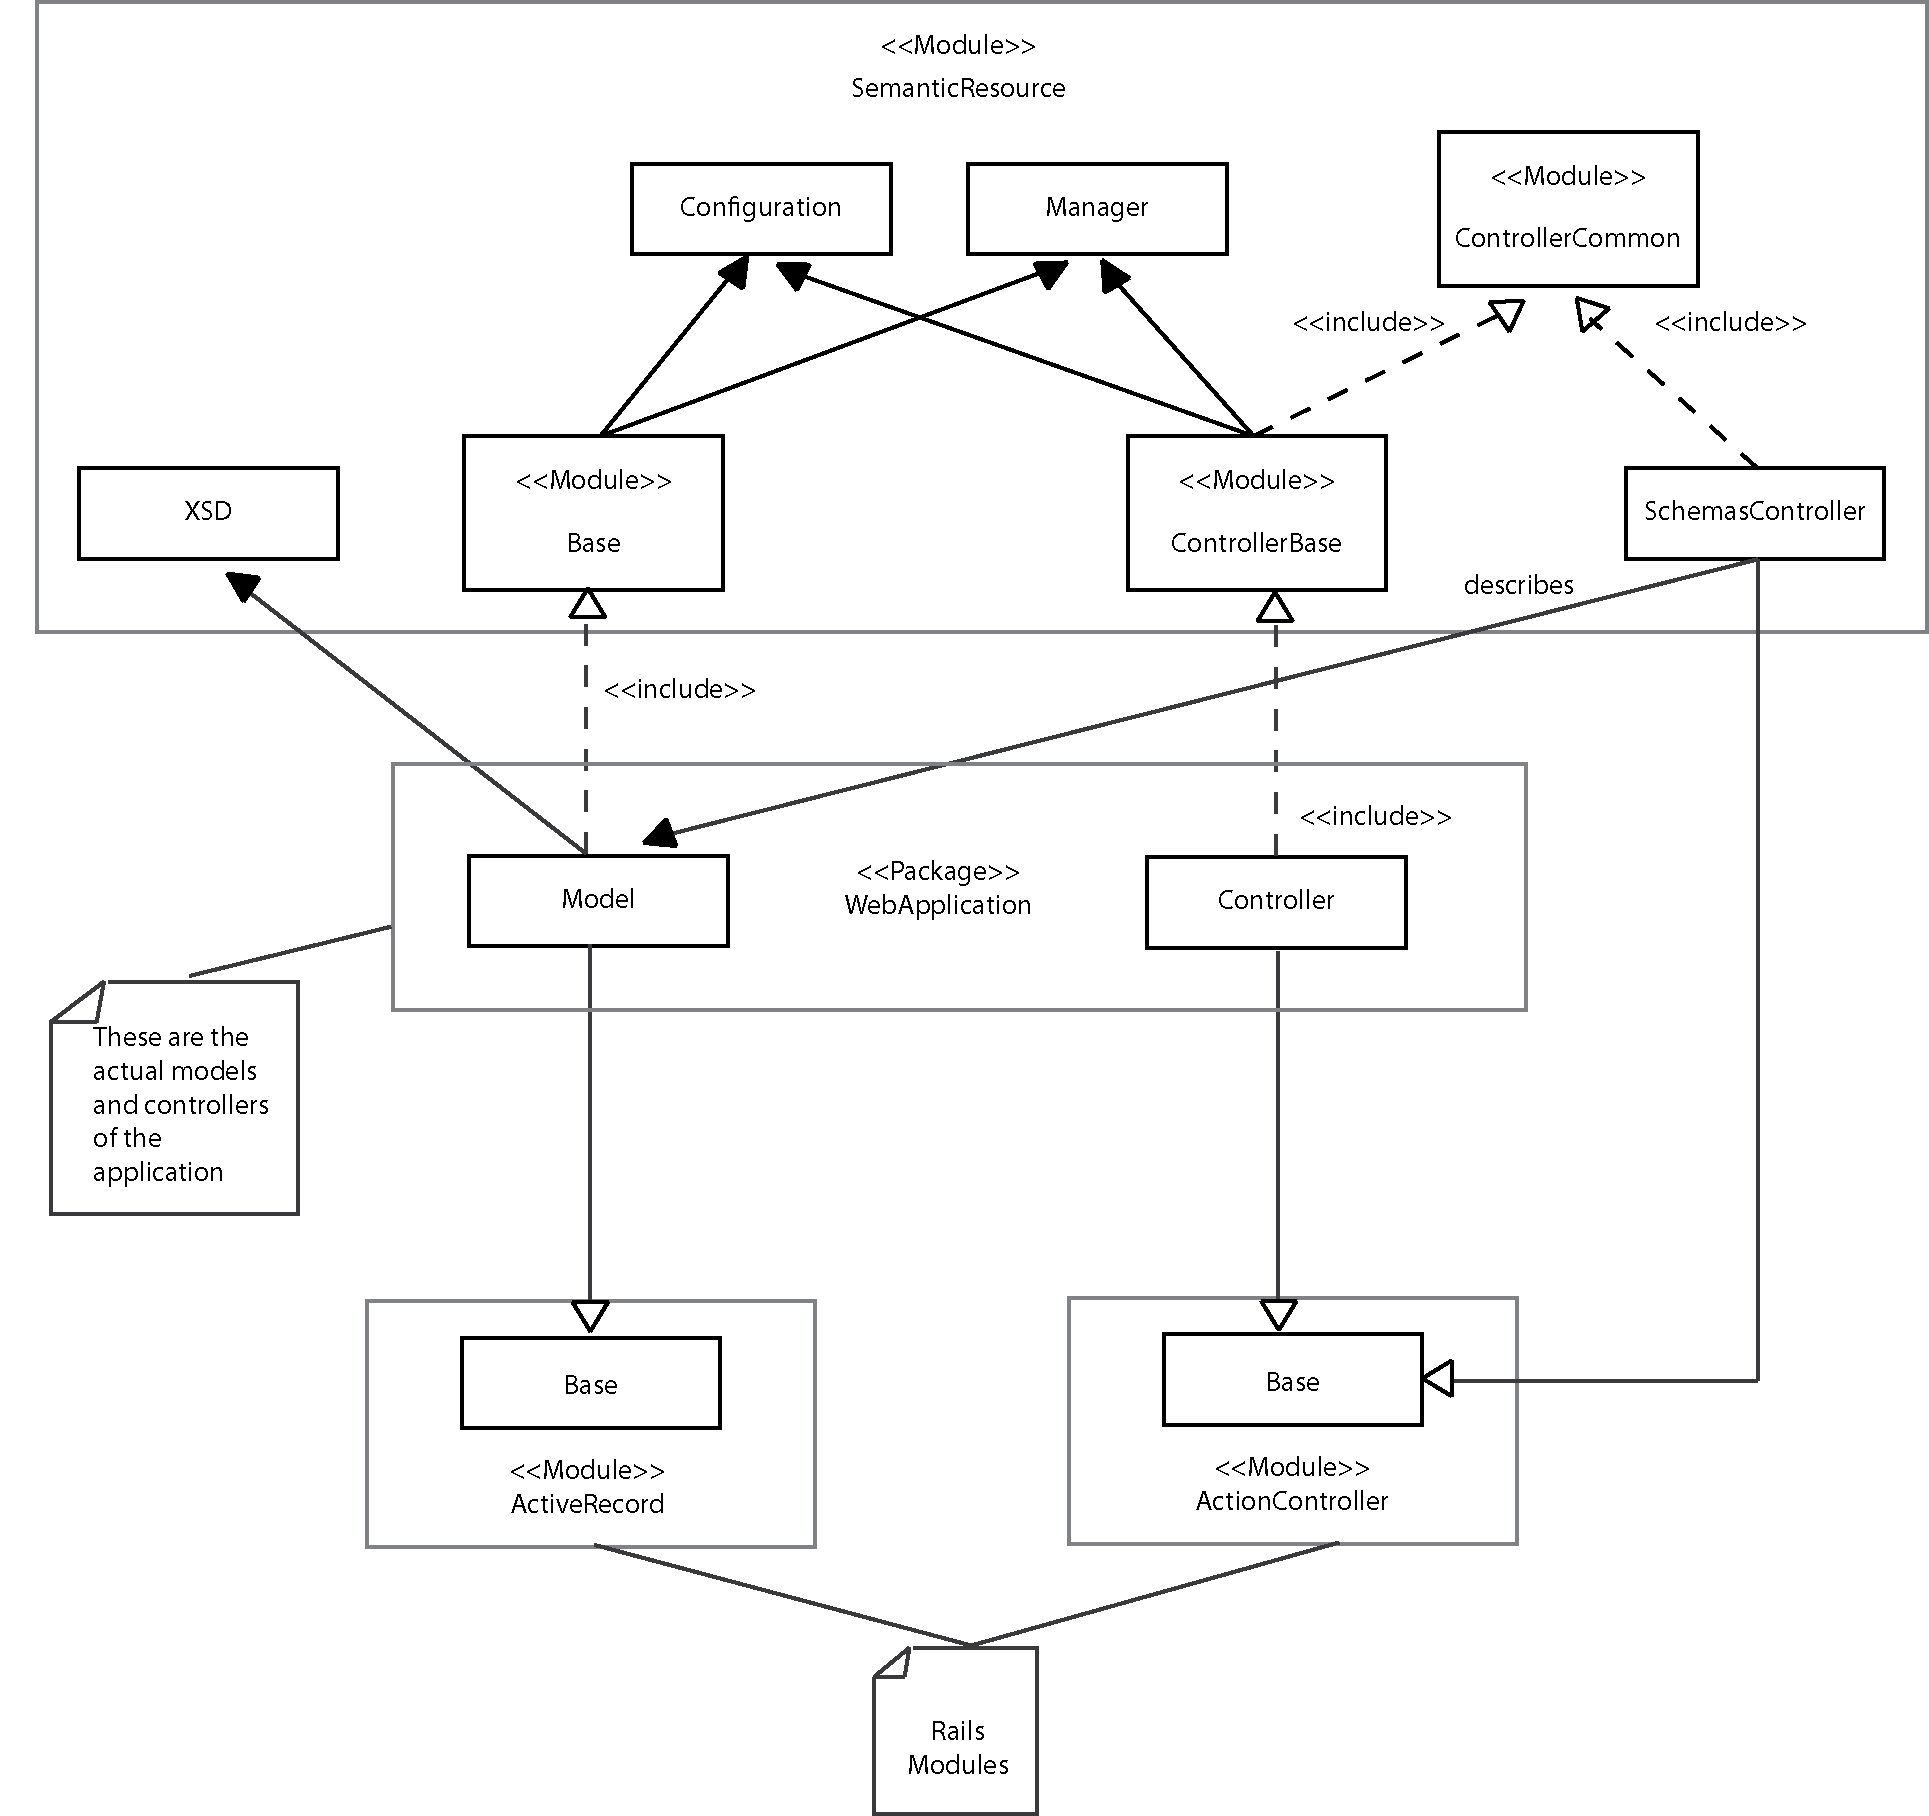
\includegraphics{SemanticRest.png}
\end{tabularx}}
\caption{Main architectural blocks of the Semantic REST library}
\end{table}


\item \texttt{SemanticResource::ControllerBase} is a module analog to\\  \texttt{SemanticResource::Base} that can be included
  in another core component of the Ruby on Rails framework an \texttt{ActionController:: Base} controller class. It extends its
  behavior with extra functionality providing default implementations for the actions of the controller answering to the REST uniform interface. These methods are the same methods of any other
  Rails RESTful controller. The methods in the module provide a default behavior involving the retrieval of the resource
  graph, the selection of the response representation and the rendering of the answer. The developer can decide to
  overwrite these methods providing his own implementation for some part of this logic, or replacing the whole method.
\item \texttt{SemanticResource::SchemasController} is a Ruby class object inheriting from the Ruby on Rails controller
  class \texttt{ActionController:: Base} that behaves as a normal Ruby on Rails controller but offering the description
  of the meta data of all the Semantic RESTful services defined in the web application. For every
  \texttt{SemanticResource::Base} class in the application, the \texttt{SemanticResource::SchemasController} controller
  gives access to the service description, model triplets, lifting and lowering operations describing the
  resource. These representations are generated dynamically by the \texttt{SemanticResource:: SchemasController}
  controller using the meta programming features of Ruby.
\item \texttt{SemanticResource::Manager} is a class that provides runtime registration functionality for the RESTful semantic
  resources defined in the application. It can receive methods from other objects querying which resources, models or
  lowering operations are registered in the application. New objects can be registered or unregistered at run time.
\item \texttt{SemanticResource::ViewHelpers} is module that contains methods that can be used by the developer in the
  creation of a HTML representation of a semantic RESTful web service, to generate HTML tags with RDFa or micro formats
  semantic annotations. These methods can be used together with the regular Ruby on Rails view helpers in the edition of
  view templates.
\item \texttt{SemanticResource::ControllerCommon} is a module contained some factored functionality used in
  the \texttt{SemanticResource::ControllerBase} module and the \texttt{SemanticResource::SchemasController} class.
\item \texttt{SemanticResource::Configuration} is a class that holds methods that configure some aspects of the
  behavior of the SemanticREST library as the default HTML representation for the resources (RDFa or HTML with
  micro formats) or alias for URIs namespaces.
\item \texttt{routing.rb} This file contains some methods of the SemanticResource module that allows an easy insertion
  of a \texttt{SemanticResource:: SchemasController} controller in the routing mechanism for requests of Ruby on Rails.
\item \texttt{SemanticResource::RestfulJsonpMiddleware} is class that implements a Ruby Rack middleware that can be
  plugged into the Ruby on Rails compliant Rack middlewares stack allowing JSONP requests with all the HTTP methods.
\item \texttt{SemanticResource::XSD} a class for easy use of XML Schema data types in the description of RESTful semantic resources.
\end{itemize}

\subsection{Practical creation of a RESTful semantic web service with Semantic REST}

In this section we will describe each component of the library through a practical example where a RESTful
semantic web service is built using the Semantic REST library.

\subsubsection{Defining the resource Model}
The starting point in the design of a new RESTful semantic resource with Semantic REST is the definition of a semantic
model. The output of this definition is a RDF graph that describes a RDF class using RDF Schema properties. In the
example the description of the resource will be inserted into an existing Ruby on Rails \texttt{ActiveRecord} simple model
modeling a book.\\

This model is defined in the \texttt{Book} class that is related to a SQL table \texttt{books} whose columns correspond
to the properties of the \texttt{Book} model.

The listing \ref{books_migration} shows the Rails migration that creates the \texttt{books} SQL table.

\begin{table}
\vspace{5 mm}
\begin{lstlisting}
class CreateBooks < ActiveRecord::Migration
  def self.up
    create_table :books do |t|
      t.string :title
      t.date :published
      t.string :category
      t.integer :pages
      t.string :isbn
      t.string :editorial
      t.timestamps
    end
  end

  def self.down
    drop_table :books
  end
end
\end{lstlisting} 
\vspace{5 mm}
\caption{Migration for the SQL books table}
\label{books_migration}
\end{table}

Provided this regular Ruby on Rails model, in order to convert it into a semantic model, it is only required to include
the \texttt{SemanticResource::Base} module and to define a namespace for the resource, as shown in the code of
\ref{define_res_1}.

\begin{table}
\vspace{5 mm}
\begin{lstlisting}
require 'semantic_resource/base'

class Book < ActiveRecord::Base

  include SemanticResource

  set_resource_namespace :test, "http://test.com"

end
\end{lstlisting} 
\vspace{5 mm}
\caption{Initial definition of the Book resource}
\label{define_res_1}
\end{table}

With this code we have inserted the \texttt{SemanticResource::Base} module into the \texttt{Book} class and provided a
default namespace for the resource, in this case \texttt{http://test.com}. With this minimal definition we can already
retrieve the RDF graph for this semantic model. The listing \ref{book_show1} shows the result of an invocation sending
the message \texttt{to\_rdf} to the \texttt{Book} object.

\begin{table}
\vspace{5 mm}
\begin{lstlisting}
>> Book.to_rdf
Book.to_rdf
=> "@prefix rdf: <http://www.w3.org/1999/02/22-rdf-syntax-ns#> .\n@prefix rdfs: <http://www.w3.org/2000/01/rdf-schema#> .\n@prefix xsd: <http://www.w3.org/2001/XMLSchema#> .\n<http://localhost:3000/schemas/models/Book> <http://www.w3.org/1999/02/22-rdf-syntax-ns#type> rdfs:Class .\n<http://semantic_rest/siesta#id> <http://www.w3.org/1999/02/22-rdf-syntax-ns#type> rdfs:Property .\n<http://semantic_rest/siesta#id> rdfs:domain <http://localhost:3000/schemas/models/Book> .\n<http://semantic_rest/siesta#id> rdfs:range rdfs:Datatype .\n<http://test.com#category> <http://www.w3.org/1999/02/22-rdf-syntax-ns#type> rdfs:Property .\n<http://test.com#category> rdfs:domain <http://localhost:3000/schemas/models/Book> .\n<http://test.com#category> rdfs:range <http://www.w3.org/2001/XMLSchema#string> .\n<http://test.com#pages> <http://www.w3.org/1999/02/22-rdf-syntax-ns#type> rdfs:Property .\n<http://test.com#pages> rdfs:domain <http://localhost:3000/schemas/models/Book> .\n<http://test.com#pages> rdfs:range <http://www.w3.org/2001/XMLSchema#integer> .\n<http://test.com#title> <http://www.w3.org/1999/02/22-rdf-syntax-ns#type> rdfs:Property .\n<http://test.com#title> rdfs:domain <http://localhost:3000/schemas/models/Book> .\n<http://test.com#title> rdfs:range <http://www.w3.org/2001/XMLSchema#string> .\n<http://test.com#isbn> <http://www.w3.org/1999/02/22-rdf-syntax-ns#type> rdfs:Property .\n<http://test.com#isbn> rdfs:domain <http://localhost:3000/schemas/models/Book> .\n<http://test.com#isbn> rdfs:range <http://www.w3.org/2001/XMLSchema#string> .\n<http://test.com#editorial> <http://www.w3.org/1999/02/22-rdf-syntax-ns#type> rdfs:Property .\n<http://test.com#editorial> rdfs:domain <http://localhost:3000/schemas/models/Book> .\n<http://test.com#editorial> rdfs:range <http://www.w3.org/2001/XMLSchema#string> .\n<http://test.com#published> <http://www.w3.org/1999/02/22-rdf-syntax-ns#type> rdfs:Property .\n<http://test.com#published> rdfs:domain <http://localhost:3000/schemas/models/Book> .\n<http://test.com#published> rdfs:range <http://www.w3.org/2001/XMLSchema#date> .\n"
\end{lstlisting} 
\vspace{5 mm}
\caption{Initial definition of the Book resource}
\label{book_show1}
\end{table}

In the lising \ref{book_show1} some default choices made by the code o the Semantic REST
library can be also noted. First of all, the semantic model RDF class has been assigned the name of the class combined with the base URI of the
application (in this case localhost and default port) and the route to the schemas controller, as will be later
explained. The RDF properties have been created extracting dynamically the names of the properties from the Book class and
combining them with the defined URI for the resource \texttt{http://test.com}. The type of these RDF properties have
been automatically assigned mapping the SQL type of the SQL table column to a Xml Schema type. A special property has been
added for the primary key column. This column is mandatory in Rails to identify the instances of the \texttt{Book} class
and is also treated in a special way by Semantic REST. \\
This default mapping is not necessarily the final desired description of the model. Imagine, for instance,
that it is desired to change the properties by properties from the Dublin Core (\url{dublincore.org/}) ontology, or to change the data type of the properties. This can be achieved using a set of of annotations from  the
\texttt{SemanticResource::Base} model, as is shown in the code from \ref{book_show2}

\begin{table}
\vspace{5 mm}
\begin{lstlisting}
require 'semantic_resource/base'

class Book < ActiveRecord::Base

  include SemanticResource

  set_resource_namespace :dc, "http://purl.org/dc/terms"

  set_resource_mapping do |resource|
    resource[:title] = {:uri =>[:dc, "/title"], :optional => true }

    resource[:published] = {:uri => [:dc, "/created"], :optional => true, :datatype => :dateTime}

    resource[:category] = {:uri => [:dc,"/type"], :optional => true}

    resource[:pages] = {:uri => [:dc, "/extent"], :optional => true}

    resource[:isbn] = {:uri => [:dc, "/identifier"], :optional => true}

    resource[:editorial] = {:uri => [:dc, "/publisher"], :optional => true}
  end

end
\end{lstlisting} 
\vspace{5 mm}
\caption{Definition of a semantic model with annotations}
\label{book_show2}
\end{table}

The \texttt{set\_resource\_mapping} message allows to define annotations for each property of the
model class, specifying the URI of the property, its data type, etc.\\

This description of the resource also allows to obtain RDF graph descriptions of the instances of the RDF clas. The
listing \ref{create_book1} shows how a new \texttt{Book} instance is created and its RDF graph is obtained. This time a
different encoding for the RDF graph is obtained passing a different parameter to the \texttt{to\_rdf} message. N3, RDF/XML, XHTML/RDFa, HTML with micro formats and JSON are the supported encodings.

\begin{table}
\vspace{5 mm}
\begin{lstlisting}
>> sicp = Book.create(:title => "Structure and Interpretation of Computer Programs (2nd edition)", :published => "2005",
:category => "Computer Science", :pages => 684,  :isbn => "8173715270", :editorial => "Universities Press ")

=> #<Book id: 513, title: "Structure and Interpretation of Computer Programs (...", published: nil, category: "Computer
Science", pages: 684, isbn: "8173715270", editorial: "Universities Press ", created_at: "2009-08-15 17:46:36",
updated_at: "2009-08-15 17:46:36">

>> sicp.to_rdf({:controller => "books"})

=> "@prefix rdf: <http://www.w3.org/1999/02/22-rdf-syntax-ns#> .\n@prefix rdfs: <http://www.w3.org/2000/01/rdf-schema#> .\n@prefix xsd: <http://www.w3.org/2001/XMLSchema#> .\n<http://localhost:3000/books/513> <http://www.w3.org/1999/02/22-rdf-syntax-ns#type> <http://localhost:3000/schemas/models/Book> .\n<http://localhost:3000/books/513> <http://semantic_rest/siesta#id> \"513\" .\n<http://localhost:3000/books/513> <http://purl.org/dc/terms/extent> \"684\".\n<http://localhost:3000/books/513> <http://purl.org/dc/terms/identifier> \"8173715270\".\n<http://localhost:3000/books/513> <http://purl.org/dc/terms/publisher> \"Universities Press \".\n<http://localhost:3000/books/513> <http://purl.org/dc/terms/title> \"Structure and Interpretation of Computer Programs (2nd edition)\".\n<http://localhost:3000/books/513> <http://purl.org/dc/terms/type> \"Computer Science\".\n"
\end{lstlisting} 
\vspace{5 mm}
\caption{RDF graph for a model instance}
\label{create_book1}
\end{table}

\subsubsection{Configuring the schemas controller}
Once we have defined our ontology of RDF classes and properties, annotating the classes in the model layer of Ruby on
Rails, and that we can also create instances of these classes, it is possible to allow clients to retrieve this
definitions from the web.\\
To allow the exposition of these data, the Semantic REST framework provides the
\texttt{SemanticResource::SchemasController} class. 
This class contains the full implementation of a Ruby on Rails controller with the logic required to return the
information about the services, models, lowering and lifting operations registered in the application. This information
is retrieved at run time from the \texttt{SemanticResource::Manager} class of the Semantic REST framework.

In order to provide a schemas controller for the application, the user must add one controller to the application
inheriting from \texttt{SemanticResource:: SchemasController} as shown in the code of \ref{schemas_controller_1}

\begin{table}
\vspace{5 mm}
\begin{lstlisting}
class MySchemasController < SemanticResource::SchemasController
end
\end{lstlisting} 
\vspace{5 mm}
\caption{RDF graph for a model instance}
\label{schemas_controller_1}
\end{table}

Once this new controller has been added to the application, it is necessary to route the requests for the different kind
of meta data to the controller. The Semantic REST library provides a helper function for adding these routes to the Ruby
on Rails router: \texttt{SemanticResource.draw\_routes \_to\_semantic\_controller}. The listing \ref{routing_1} shows
how the routes for the controller can be added passing the name of the schemas controller to the function.

\begin{table}
\vspace{5 mm}
\begin{lstlisting}
ActionController::Routing::Routes.draw do |map|

  # schemas controller
  SemanticResource.draw_routes_to_semantic_controller(map,'my_schemas')

  # Rails default routes
  map.connect ':controller/:action/:id'
  map.connect ':controller/:action/:id.:format'
end
\end{lstlisting} 
\vspace{5 mm}
\caption{RDF graph for a model instance}
\label{routing_1}
\end{table}

The presence of a schemas controller is entirely optional, but when not present into the application the clients need
to know beforehand the information usually provided by the schemas controller.\\

Once configured, we can start the Ruby on Rails application and ask the schemas controller for the Book class model. By
default, the route to the schemas controller is at \texttt{/schemas}, so, for instance, the route to the Book model would
be \texttt{/schemas/models/Book}. A semantic client can already consume this service. The image \ref{res_moz_1} shows
the MIT tabulator plugin (\url{http://dig.csail.mit.edu/2005/ajar/ajaw/tab.html}) for Mozilla Firefox consuming the Book model RDF graph and rendering its representation.

\begin{table}{h!}
\noindent\makebox[\textwidth]{%
\begin{tabularx}{1.2\textwidth}{XX}
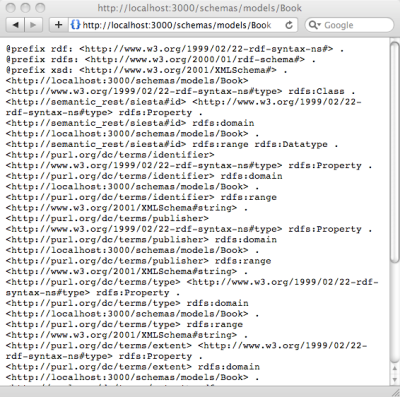
\includegraphics{resource_class.png}
\end{tabularx}}
\caption{The defined Book model RDF graph served from the schemas controller}
\end{table}


\begin{table}{h!}
\noindent\makebox[\textwidth]{%
\begin{tabularx}{1.2\textwidth}{XX}
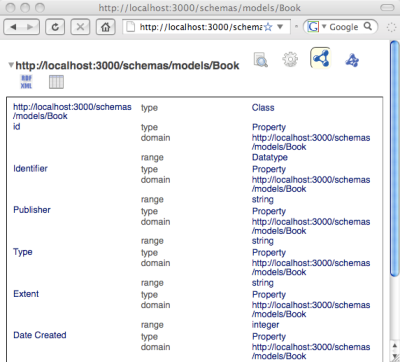
\includegraphics{moz_res_1.png}
\end{tabularx}}
\caption{The defined Book model RDF graph consumed by the Tabulator plugin}
\label{res_moz_1}
\end{table}

\subsubsection{Building the RESTful service}

A RESTful semantic web service is defined not only by a graph containing the resource and the resource class model, but also
for the logic that modifies the state of the resource along with the design principles of the REST uniform interface. All
this information: RDF triples of the resource, REST interface plus lowering and lifting mechanisms will be exposed by
the schemas controller as a extended hRESTS service description.\\
The REST interface to the resource is built with Semantic REST extending the Rails RESTful controllers classes with the
\texttt{SemanticResource:: ControllerBase} module. This module implements all the logic needed to expose the RDF graphs of the resources according to REST semantics.\\
The code in \ref{books_controller_1} shows how to build a controller for the \texttt{Book} class defined in previous
sections.

\begin{table}
\vspace{5 mm}
\begin{lstlisting}
require 'semantic_resource'

class BooksController < ApplicationController
  include SemanticResource::ControllerBase
end
\end{lstlisting} 
\vspace{5 mm}
\caption{Books controller}
\label{books_controller_1}
\end{table}

The controller also needs to be inserted into Ruby on Rails routes as any other controller of the application. The code
in \ref{routing_2} shows the required code.

\begin{table}
\vspace{5 mm}
\begin{lstlisting}
ActionController::Routing::Routes.draw do |map|

  # Books controller
  map.resources :books

  # schemas controller
  SemanticResource.draw_routes_to_semantic_controller(map,'my_schemas')

  # Rails default routes
  map.connect ':controller/:action/:id'
  map.connect ':controller/:action/:id.:format'
end
\end{lstlisting} 
\vspace{5 mm}
\caption{Routing for the Books controller}
\label{routing_2}
\end{table}

In many cases, we don't want to provide all the methods of the HTTP uniform for a certain resource. We may also decide to serve
the semantic meta data from a different controller than the controller used in the HTML of the application, maybe dued to the
different requests load that an API and a regular web application must handle. All this configuration is set up in
the Semantic REST framework as additional annotations to the resource model. It is also possible to define additional input
messages for the service or change the parameters of the URI, according to the extended hRESTS specification.\\
The code in \ref{book_3} shows how this configuration can be tuned.

\begin{table}
\vspace{5 mm}
\begin{lstlisting}
require 'semantic_resource/base'

class Book < ActiveRecord::Base

  include SemanticResource

  set_resource_namespace :dc, "http://purl.org/dc/terms"

  set_resource_mapping do |resource|
    resource[:title] = {:uri =>[:dc, "/title"], :optional => true }
    resource[:published] = {:uri => [:dc, "/created"], :optional => true, :datatype => :dateTime}
    resource[:category] = {:uri => [:dc,"/type"], :optional => true}
    resource[:pages] = {:uri => [:dc, "/extent"], :optional => true}
    resource[:isbn] = {:uri => [:dc, "/identifier"], :optional => true}
    resource[:editorial] = {:uri => [:dc, "/publisher"], :optional => true}
  end

  # operations for the Books service
  define_index_operation(:controller => 'books', :action => 'index')
  define_show_operation(:controller => 'books', :action => 'show')
  define_create_operation(:controller => 'books', :action => 'create')
  define_destroy_operation(:controller => 'books', :action => 'destroy')
  define_update_operation(:controller => 'books', :action => 'update')

end
\end{lstlisting} 
\vspace{5 mm}
\caption{Routing for the Books controller}
\label{book_3}
\end{table}

Once this information is added we can already consume the service description from the schemas controller. By default
this information will be available at the URI \texttt{/schemas/services/BookService}. The figure \ref{book_service_1}
shows how this information is accessed from the browser. Since Semantic REST supports micro formatted HTML and RDFa
embedded into HTML, the RDF graph can be requested embedded into a HTML page at the URI
\texttt{/schemas/services/BookService.html}. By default XHTML with RDFa will be the chosen encoding. The
figure \ref{book_service_2} shows this version of the graph. This is a nice way to provide automatic documentation of
the set of services in the API of a web application.

\begin{table}{h!}
\noindent\makebox[\textwidth]{%
\begin{tabularx}{1.2\textwidth}{XX}
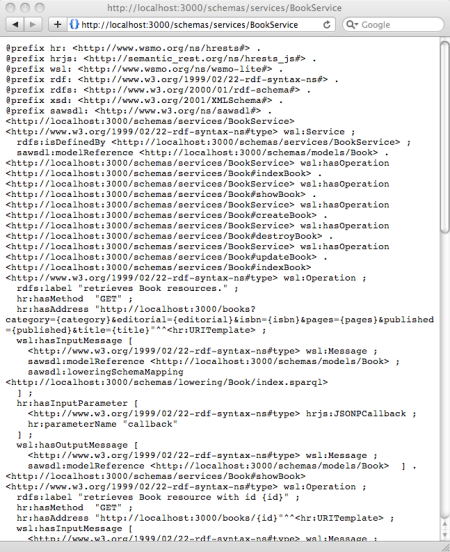
\includegraphics{book_service1.png}
\end{tabularx}}
\caption{The Book RESTful semantic service description}
\label{book_service_1}
\end{table}


\begin{table}{h!}
\noindent\makebox[\textwidth]{%
\begin{tabularx}{1.2\textwidth}{XX}
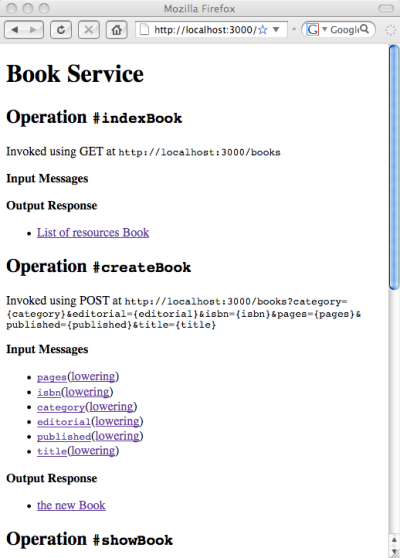
\includegraphics{book_service2.png}
\end{tabularx}}
\caption{RDFa encoded version of the Book Service}
\label{book_service_2}
\end{table}


As part of the service description, Semantic REST also generates SPARQL queries for the lowering mechanism of the
resource. These queries use the information provided as semantic annotations in the model class. Those attributes
marked as optional, will be also optional in the lowering SPARQL query. The listing \ref{sparql_1} shows the lowering
query for the create operation of the defined \texttt{BookService}. 

\begin{table}
\vspace{5 mm}
\begin{lstlisting}
SELECT ?pages ?isbn ?category ?editorial ?published ?title  WHERE {
  OPTIONAL { ?x <http://purl.org/dc/terms/extent> ?pages .  } 
  OPTIONAL { ?x <http://purl.org/dc/terms/identifier> ?isbn .  } 
  OPTIONAL { ?x <http://purl.org/dc/terms/type> ?category .  } 
  OPTIONAL { ?x <http://purl.org/dc/terms/publisher> ?editorial .  } 
  OPTIONAL { ?x <http://purl.org/dc/terms/created> ?published .  } 
  OPTIONAL { ?x <http://purl.org/dc/terms/title> ?title .  }  
}
\end{lstlisting} 
\vspace{5 mm}
\caption{Routing for the Books controller}
\label{routing_1}
\end{table}

The Semantic REST library also offers the possibility to the user of customizing the behavior of the resources
controller. This can be achieved overwriting part or the whole default implementation of the standard Ruby on Rails
REST methods, provided by the Semantic REST library.\\
In the code at \ref{overwriting_book_controller} the behavior of the controllers is modified by filtering the
books by a hypothetical \texttt{released} attribute that states if the book has already been released. In order to
retrieve the resource in the filter method the message \texttt{semantic\_find} from the Semantic REST
\texttt{SemanticResource::ControllerBase} module is used. This method encapsulates the logic to interpret the lowered
request for the resource. Other methods encapsulating other parts of the controller behavior are also available and the
developer can mix them with his own logic to modify the standard behavior of the library.

\begin{table}
\vspace{5 mm}
\begin{lstlisting}
require 'semantic_resource'

class BooksController < ApplicationController  
  
  include SemanticResource::ControllerBase

  before_filter { head(400) unless semantic_find.released }

end
\end{lstlisting} 
\vspace{5 mm}
\caption{Books controller}
\label{overwriting_bok_controller}
\end{table}

\subsubsection{JSONP request}

The proposed extensions to the hRESTS specification provides special RDF properties to allow a client to send JSONP
requests to the server with extra parameters providing the right HTTP method of the request, since JSONP requests can
only be sent in HTTP GET requests. Ruby on Rails provides a similar mechanism for specifying a
\texttt{method} parameter in the requests to simulate PUT and DELETE requests from a web browser. Unfortunately this
mechanism only works with POST requests, rendering it useless for JSONP GET requests.\\
To solve this problem the Semantic REST library implements a Rack (\url{http://rack.rubyforge.com}) middleware that can be plugged into the Ruby on
Rails Rack middleware stack to modify the way Rails handles the request. It allows the overwriting of the method in GET
requests. Rack is a standard interface between web servers and Ruby web frameworks that defines a stable interface for
the HTTP request and response. Different Ruby classes can be stacked for processing requests.\\

To enable this middleware it must be inserted into the environment configuration file of the Ruby on Rails
application. Enabling this feature nevertheless must be carefully thought since it has important security implications
for the application. Using Rack middlewares is also only possible for versions of Rails posterior to Ruby on Rails 2.3,
since previous versions were not Rack compliant. A workaround for solving this issue is also provided with the library
and should work with Rails 2.X versions, but it may not work properly in some cases since it relies in Rails messages
not belonging to the public Rails API.

\subsubsection{Description of external services}\label{desc_ext_servs}

The hRESTS specification allows the description of any RESTful web service. Specifications for services from an external
application can also be provided if they can be described with the
hRESTS ontology and proposed extensions. Thus any hRESTS compliant client will be able to consume the service even if the original
provider does not support the hRESTS specification.\\
Semantic REST provides an easy way for authoring hRESTS description of external services and its integration into the
application based in the description of the services using YAML files. YAML is the default format for writing configuration
files in Ruby on Rails so it is well known by Ruby on Rails developers. In the chapter \ref{capituloTS} of this document
a YAML description of a Twitter service was provided as an example. For the schemas controller to serve this
specifications, the YAML descriptions of the services must be stored in some path of the application files and the path
to this directory configured in the application using the functions from the \texttt{SemanticResource::Configuration}
module. Once this configuration is finished, the schemas controller will automatically search in that directory for a
YAML file matching the requested service and will transform it into a RDF graph encoded with the requested representation:
N3, RDF/XML, XHTML/RDFa or HTML with micro formats.\\
If the Semantic REST library is installed in the system it is also possible to use this functionality from the command
line using the hrest\_gen command.

\subsubsection{Working with relations between resources}

When designing an application or API in the terms of a set of REST resources, it is sometimes useful to establish hierarchical
relationships between resources. In this way we can specify that our Book resource may have many Chapters resources
nested, Semantic REST supports the nesting of resources with a set of specific annotations.\\ 
Services descriptions, instances triple graphs, and lowering mechanisms in SPARQL will also recognize these dependency
relations and change their content according to the provided annotations.

\subsubsection{Packaging and installation of the Semantic REST library}

The semantic REST library is available as an Open Source Ruby Gem (\url{http://rubygems.org}), the standard way of distributing Ruby libraries, that can be
easily installed from the web. The gem is hosted at Github (\url{http://github.com}) and can be installed with the command shown at
\ref{install_command}

\begin{table}
\vspace{5 mm}
\begin{lstlisting}
\sudo gem install semantic_rest-antoniogarrote --source http://gems.github.com
\end{lstlisting} 
\vspace{5 mm}
\caption{Installation of the Semantic REST gem}
\label{install_command}
\end{table}

\section{The Siesta client library}

In this section the client counterpart of the Semantic REST library for Ruby on Rails, the Siesta Javascript library,
will be described.

\subsection{Development Goals}
At the time of starting the development of the client library for consuming RESTful semantic web services, several
important design decisions had to be taken. These decisions conformed the basis of the specification of what the
client library would be. They can be summarized in the following points.

\begin{itemize}
\item the main goal of the library is granting a model layer for building Javascript applications using RESTful
  semantic web services for creating, deleting, updating and querying model objects.
\item The client of the library should run in any web browser without relaying into external services or plugins, thus
  the implementation language should be plain cross browser Javascript.
\item The client library should be able to consume hRESTS with all the extensions compliant service descriptions.
\item The client should be (along with the browser) an stand alone client for consuming RESTful semantic web services.It should not depend on any server side
  technology for consuming the services.
\item the client should not be dependent on any third party Javascript library allowing the decoupling of the core of the
  library from third parties libraries used to implement certain parts of the library.
\end {itemize}

This set of goals conforms a fairly restrictive implementation model that tries to build a minimal implementation that
can work in any web browser. Several parts of the library, like the SPARQL query engine or the parsers for different RDF
encodings, could have been extracted from the library an be provided as server side services but it would have prevented the
use of the library when these parts were not present .

Provided this development goals, a set of user stories from  point of view of the developer using the library can be
summarized in the next paragraphs.

\begin{itemize}
\item The library should provide a mechanism for defining {\it semantic classes} linked to a remote semantic RESTful web
  service.
\item This classes should provide CRUD operations (create, read, update and destroy) operations for manipulating the
  model.
\item The library should automate the description of the classes and the communication with the back end semantic RESTful
  web service through the semantic meta data exposed in the service.
\item The library should be easily inserted or used as a replacement for the model layer in other Javascript frameworks.
\end{itemize}

\subsection{Design overview}

The library have been designed as a set of layers, each one building functionality on top of the previous. These layers
provide increasing abstraction level from the lower ones. These layers are summarized in the following list:

\begin{itemize}
\item \textbf{Foundation}, providing HTTP communications, SPARQL support, parsing of semantic formats, and triples
  graph operations and repository.
\item \textbf{Service model} a set of Javascript objects modeling the RESTful semantic web services service model:
  messages, operations , models and services. These objects abstract the client layer from the concrete details in the consumption of
  RESTful semantic web services, like doing HTTP requests, parsing responses, manipulating triples in the graph and
  executing SPARQL requests.
\item \textbf{CRUD model}, the objects of this layer offers to the clients a familiar interface based in the definition
  of model classes that create, read, update and destroy remote semantic data. It hides the complexity of dealing the
  service mode layer.
\end{itemize}

\begin{table}
\noindent\makebox[\textwidth]{%
\begin{tabularx}{0.5\textwidth}{XX}
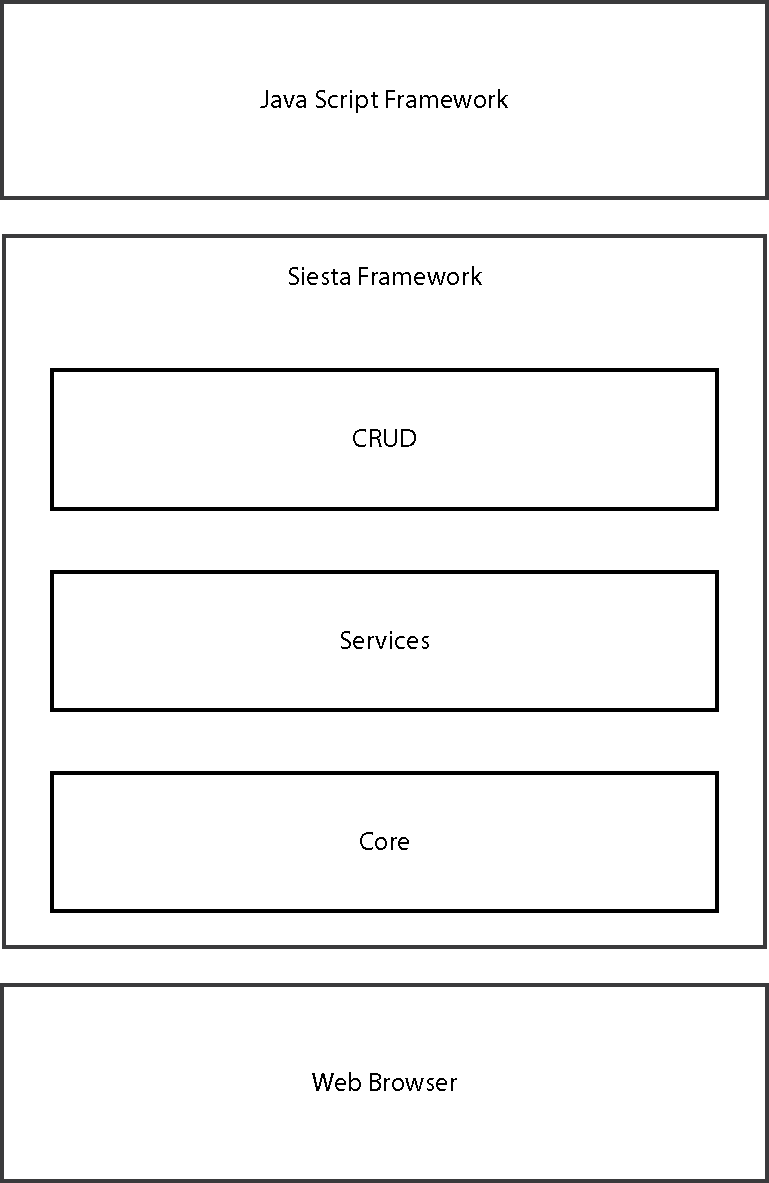
\includegraphics{siesta1.png}
\end{tabularx}}
\caption{Siesta framework layers and its relation with the browser and other frameworks}
\end{table}


\subsection{The Foundation Layer}
From the development goals previously commented it was made clear that the main design concern in the design of the foundation
layer would be its modularity. In order to implement the library in a reasonable time, it has been necessary to reuse as many libraries
implementing parts of the desired functionality as possible. But these dependencies were required to be easily removed and
changed for other libraries or back end services. To fulfill this requirement, a system of plugins have been
implemented where low level parts of the library have been encapsulated in a core library plus a set of
interface. Different libraries have been used when possible to offer this functionality. These extra libraries can be plugged
into the core library through small adapters implementing the defined interfaces. A configuration object
can be used later in conjunction with the dynamical capacities of Javascript to decide at run time which code should be
executed to accomplish a certain functionality.\\

The main objects in this layer are described next:

\begin{itemize}
\item \textbf{Core objects}, a set of objects implementing basic building blocks for that can be used by the rest of objects in
  the framework. Some examples of functions in this objects are \texttt{Siesta.registerNamespace} for defining
  namespaces in Javascript functions, \texttt{Siesta.Framework.classBuilder} for simulating classes in Javascript
  through the manipulation of the objects prototypes or \texttt{Siesta.Framework.chooseFormatterFor} containing
  heuristics for determining the format of a RDF encoding. Another set of important objects in the core module are the objects
  that define a triplets graph: \texttt{Siesta.Framework.BlankNode}, \texttt{Uri}, \texttt{Literal}, \texttt{Triple}, or
  \texttt{Graph}. These objects also provide graph operations as union, or intersection.
\item \textbf{Siesta.Utils}. This namespace registers function for different auxiliary functionality used in several
  parts of the framework, like a uniform interface to the HTML parsing capacities of the different browsers or a
  sequentializer of AJAX requests.
\item \textbf{Siesta.Events}. A notifications hub compliant with the Open AJAX Hub 2.0 specification. This mechanism
  allows asynchronous communication between Javascript objects through a publish/subscribe notifications mechanism.
\item \textbf{Siesta.Sparql} An interface defining functions for querying a SPARQL engine.
\item \textbf{Siesta.Formats.Turtle} An interface defining functions for transforming N3/Turtle documents into graphs
  of triples.
\item \textbf{Siesta.Formats.Xml} An interface defining functions for transforming RDF/XML documents into graphs of
  triples.
\item \textbf{Siesta.Formats.Rdfa} An interface for parsing RDFa documents into triple graphs
\item \textbf{Siesta.Network} An interface for functions enabling AJAX and JSONP requests.
\end{itemize}

\begin{table}{h!}
\noindent\makebox[\textwidth]{%
\begin{tabularx}{1.2\textwidth}{XX}
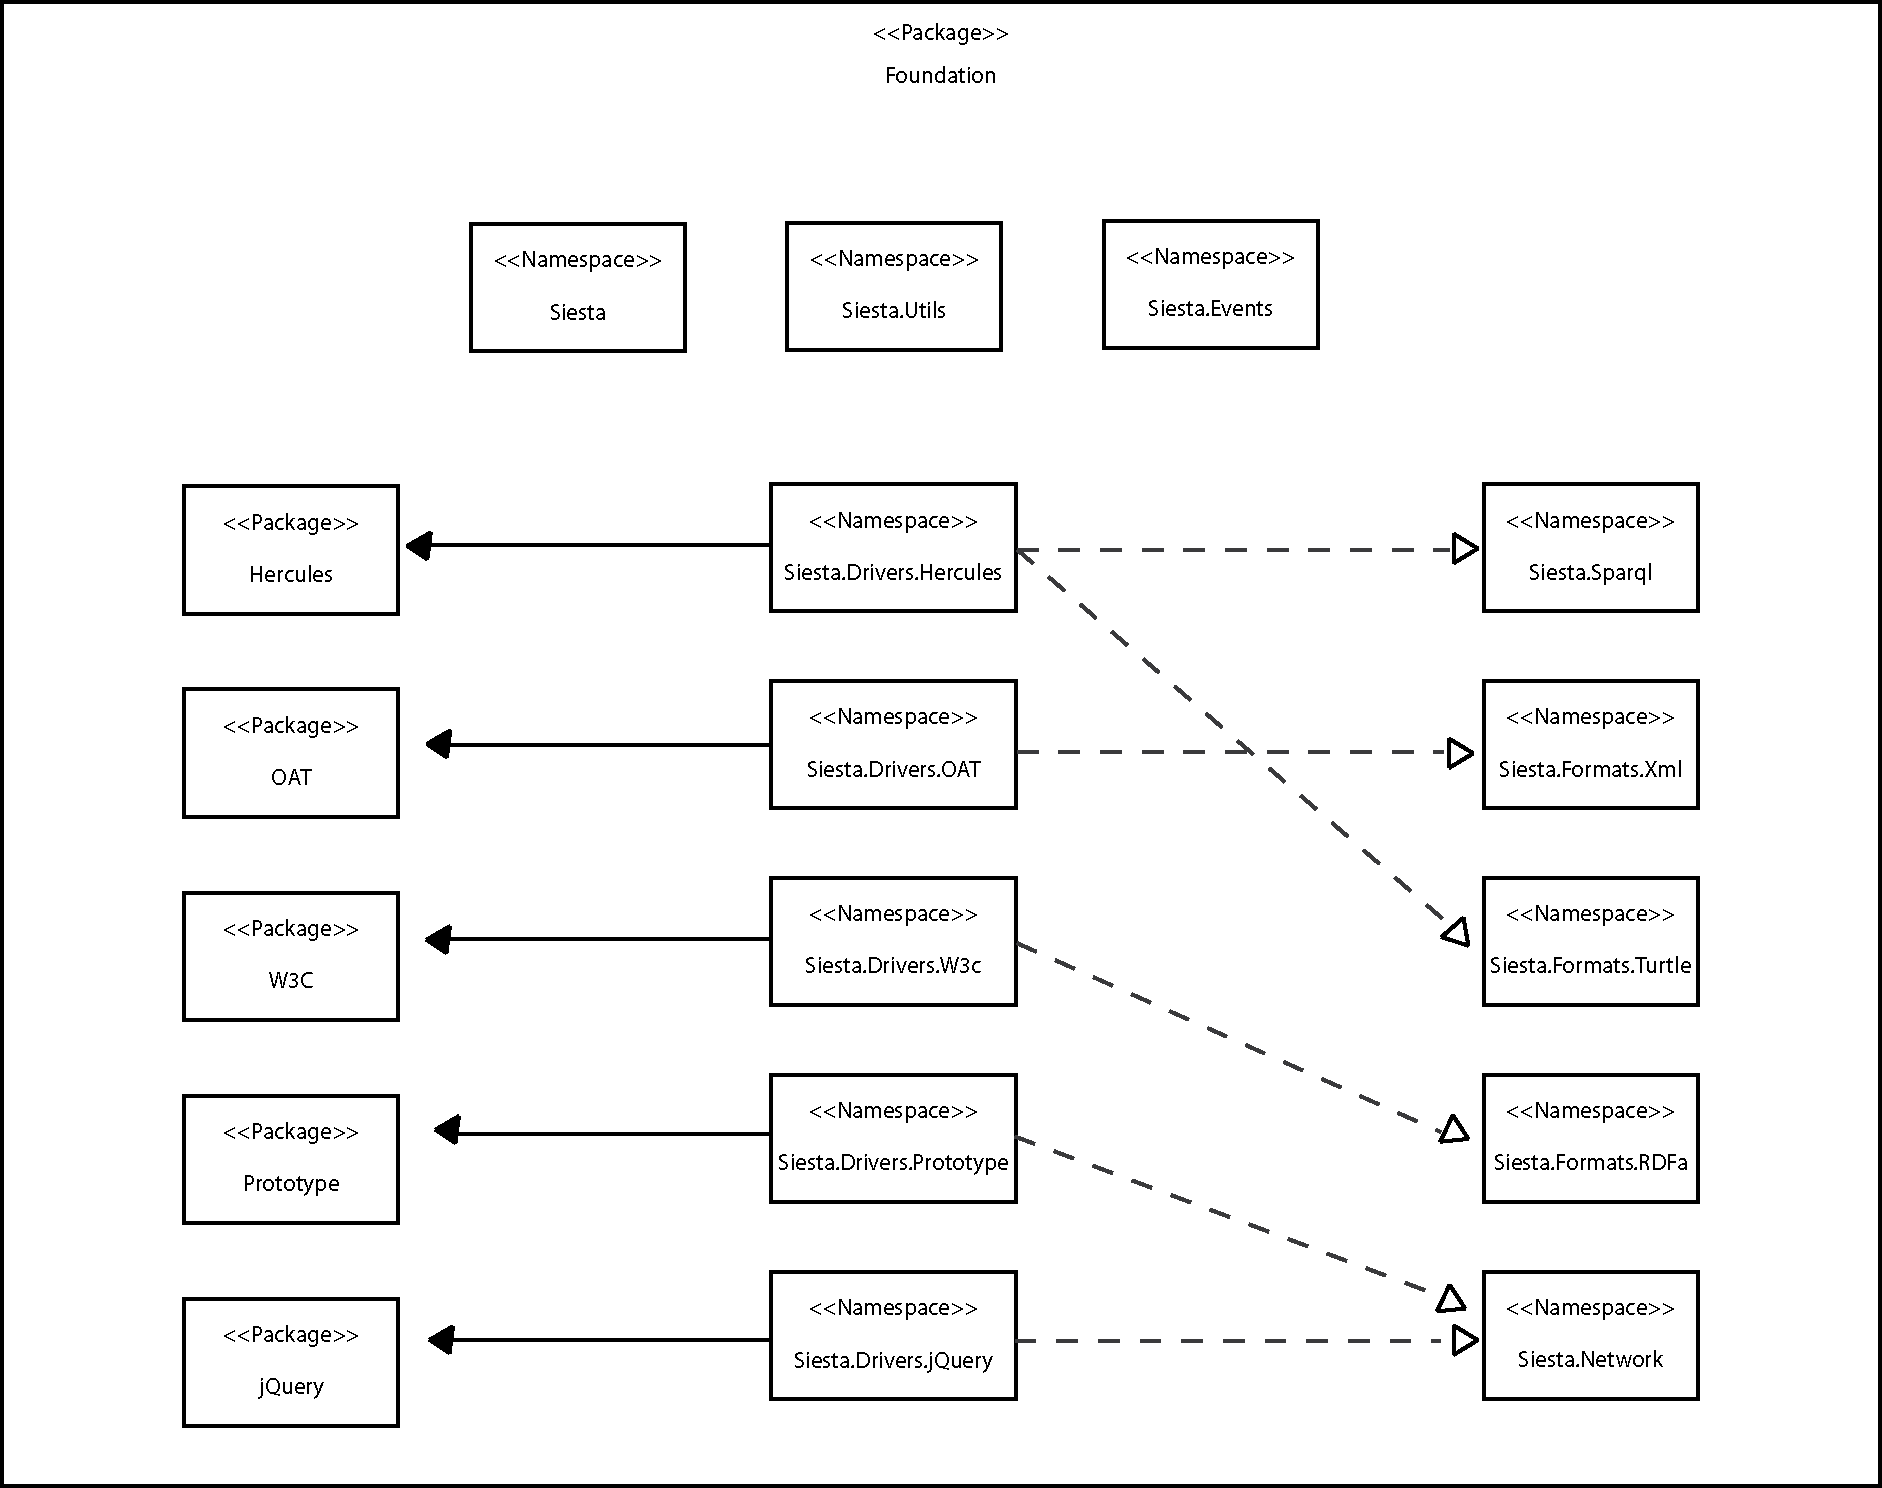
\includegraphics{siesta2.png}
\end{tabularx}}
\caption{Components in the foundation layer of the Siesta Framework}
\end{table}

In order to provide the functionalities in the namespaces \texttt{Siesta.Sparql}, \texttt{Siesta.Formats.*}, and
\texttt{Siesta.Network} different third party open source libraries have been used. To insert these libraries into the
Siesta framework, small portions of Javascript code have been written to adapt the public interfaces of these libraries to
the required interfaces defined in the Siesta framework. The libraries and implemented adapters are shown next.

\begin{itemize}
\item \texttt{Siesta.Drivers.Hercules.Sparql} a quite limited open source SPARQL engine implemented in Javascript that has been extended in different ways and inserted into
  the Siesta framework.
\item \texttt{Siesta.Drivers.Hercules.Formats.Turtle} adapter for the Turtle/N3 parser that is part of the Hercules SPARQL project.
\item \texttt{Siesta.Drivers.OAT.Formats.Xml} adapter for the RDF/XML parser part of the OAT open source project .
\item \texttt{Siesta.Drivers.W3c.Formats.Rdfa} adapter for the RDFa open source parser from the W3C.
\item \texttt{Siesta.Drivers.Prototype.network} adapter for the Prototype library network functions.
\item \texttt{Siesta.Drivers.jQuery.network} adapter for the jQuery library network functions.
\end{itemize}

Which library will be used at runtime is configured through the \texttt{Siesta.defineConfiguration} function. In
\ref{siesta_conf} a configuration for the framework is shown. When the framework is being used as a single compressed
Javascript file, this information is also used to choose which Javascript files to insert into the final Javascript
file.

\begin{table}
\vspace{5 mm}
\begin{lstlisting}
Siesta.defineConfiguration({
    drivers: ["hercules","oat","jquery","w3c"],
    sparql: "Hercules",
    formats: {
        turtle: "Hercules",
        xml: "OAT",
        rdfa: "W3c"
    },
    network: "jQuery"
});
\end{lstlisting} 
\vspace{5 mm}
\caption{Siesta framework configuration}
\label{siesta_conf}
\end{table}

\subsection{The Service Layer}

In this layer the functionality of the foundation layer is used to provide a set of objects encapsulating the logic for
consuming Semantic RESTful web services.\\

The top level object in this layer is the \texttt{Siesta.Services.Restful.Service} class. This class is initiated with a
service URI. The most important method of the class is the function \texttt{Service.connect} that starts the consumption
of the remote service. The \texttt{Service} class contains accessor methods for retrieving the components of the
service.\\

These component are the service referenced model and a set of operations. Each one of these components are modeled in
the classes \texttt{Siesta.Services.Schema} and \texttt{Siesta.Services.RestfulOperation}.\\

The \texttt{Siesta.Services.RestfulOperation} class is also composed of different objects modeling the parts of a
hRESTS operation: a set of input messages, input parameters, and an output message. It also holds the information for the address and HTTP
method of the operation. The \texttt{RestfulOperation} class offers the \texttt{RestfulOperation.consume} method that transforms a model
layer instance into a triples graph and is then lowered and sent to the remote RESTful semantic web service.\\  The \texttt{ResfulOperation} class also includes the \texttt{RestfulOperation.connect} method
into its public interface. When invoked, the object creates its component object with the information retrieved from the
server.\\

Input parameters, messages and output messages are modeled in the classes
\texttt{Siesta.Services.RestfulOperationInputParameter}, \texttt{Siesta.Services.RestfulOperationInputMessage} and
\texttt{Siesta.Services.RestfulOperationOutputMessage}. Each one of these classes provide methods into their public
interfaces for accessing to the components of the hRESTS specification: lowering and lifting mechanisms, reference models
and parameters name and values.\\

\begin{table}{h!}
\noindent\makebox[\textwidth]{%
\begin{tabularx}{1.2\textwidth}{XX}
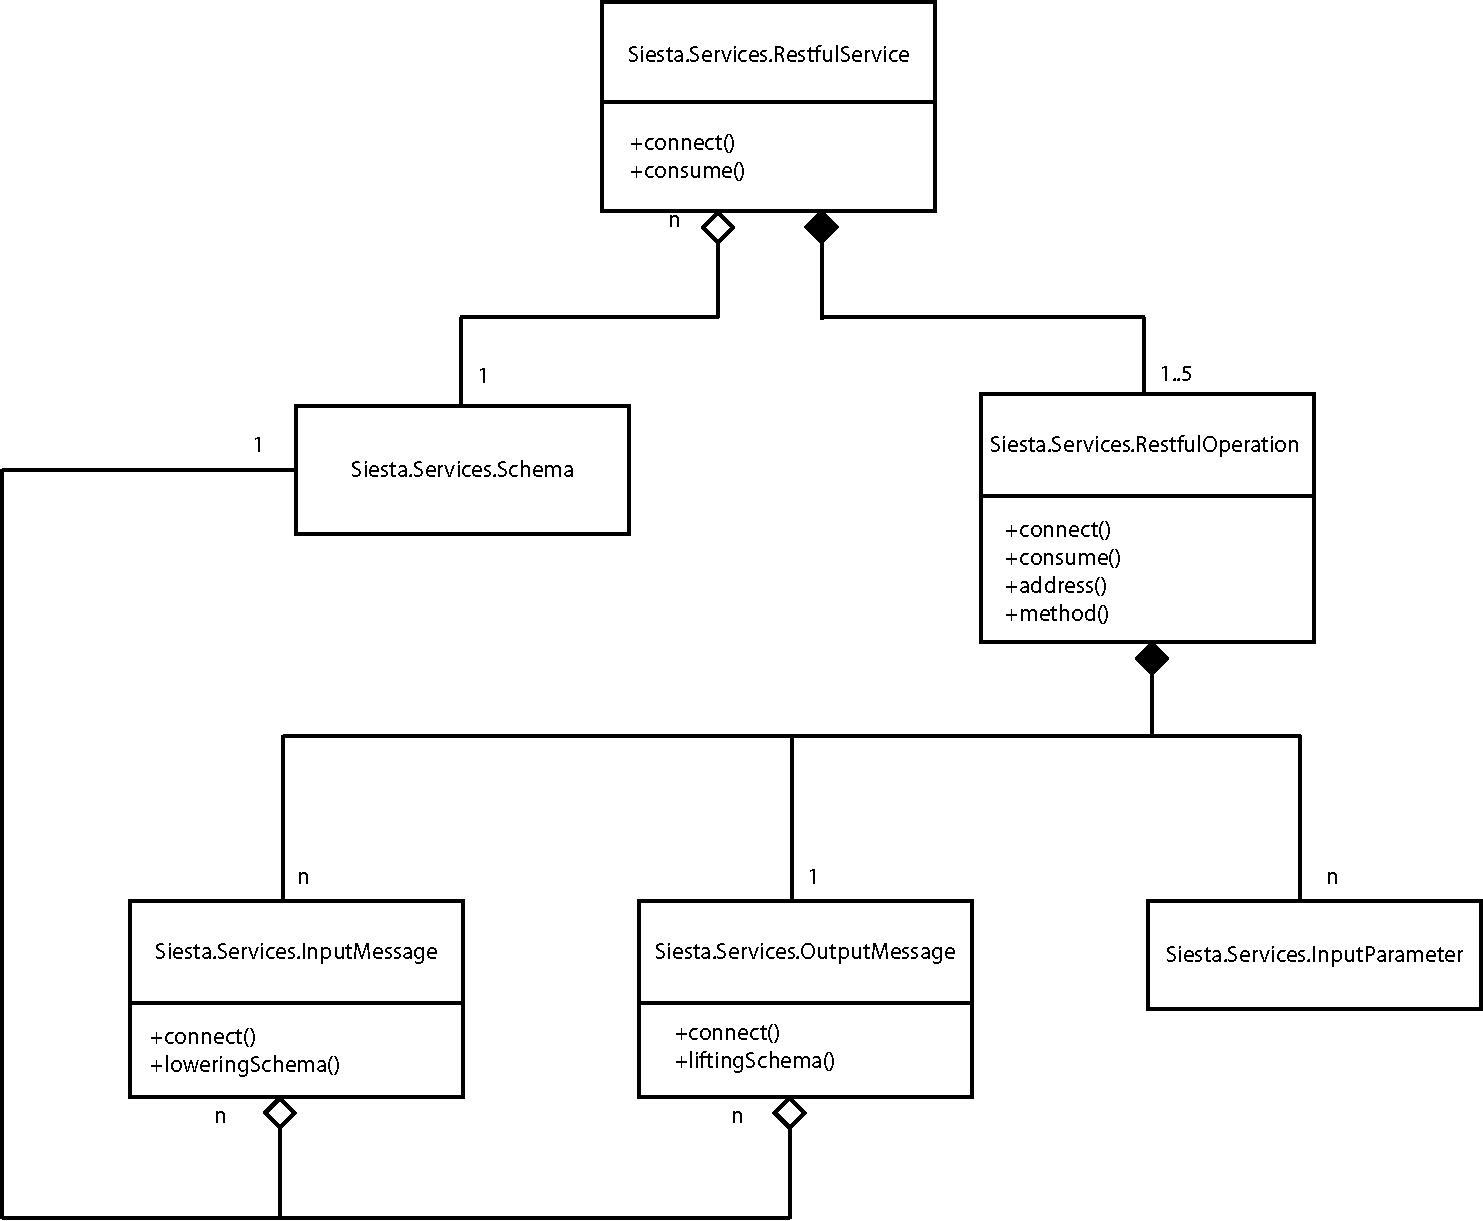
\includegraphics{siesta3.png}
\end{tabularx}}
\caption{Components in the service layer of the Siesta Framework}
\end{table}

The whole set of classes is arranged as a tree of components with the \texttt{Siesta.Services.RestfulService} class at
its top. These classes also implement a {\it builder} design patter for retrieving the components of the model
description, a call to the \texttt{ResfulService} \texttt{connect} function initiates requests to the server for
retrieving the description of the service and eventually the invocation of the \texttt{connect} method in the next level
of the tree formed by the \texttt{RestfulOperation} objects, initiating new back end requests and the invocation of the 
\texttt{connect} method of the \texttt{Siesta.Services.RestfulOperationInputParameter}, \texttt{Siesta.Services.RestfulOperationInputMessage} and
\texttt{Siesta.Services.RestfulOperationOutputMessage} objects until the full tree of components have been built.

The code in \ref{js_serv_1} shows how a \texttt{RestfulService} object consuming the \texttt{BookService} commented in
the previous section, is created, connected and invoked. Dued to the
asynchronous nature of the Javascript network mechanisms, the use of the notification mechanism is required.

\vspace{5 mm}
\begin{lstlisting}
// alias for using shorter namespaces

var evts = Siesta.Events;



//we build the service object with the URI of the 
//backend service

var uri = "http://localhost:3000/schemas/services/BookService";
var service = new Siesta.Services.RestfulService(uri);


//callback that will be invoked when the service has been successfully built

var evt = service.EVENT_SERVICE_LOADED;
var _subscription =  evts.subscribe(evt,function(event,serv,myData) {

  
  //is the event related to our service

  if(myData == service) {


    //we no longer want EVENT_SERVICE_LOADED notifications

    evts.unsubscribe(_subscription);


     //we need to find the GET opeation

     for(var _i=0; _i<serv.operations().length; _i++) {

        var op = serv.operations()[_i];
        if(op.method() == Siesta.Services.RestfulOperation.GET) {
         //this is our operation

         //we need to create the RDF graph that will be lowered

         var siestans = "http://semantic_rest/siesta'';
         var rdfsns = "http://www.w3.org/1999/02/22-rdf-syntax-ns'';
         var bookns = "http://localhost:3000/schemas/models/";

          var toLowerGraph = new  Siesta.Framework.Graph();
          var s = new Siesta.Framework.Uri("_:1");
          var p = new Siesta.Framework.Uri(siestans + "#id");
          var o = new Siesta.Framework.Literal({value: "1"});
          toLowerGraph.addTriple(new Siesta.Framework.Triple(s,p,o));
          p = new Siesta.Framework.Uri(rdfsns + "#type");
          o = new Siesta.Framework.Uri(bookns + "Book");
          toLowerGraph.addTriple(new Siesta.Framework.Triple(s,p,o);


         //we will be notified when the operation 
         //had been consumed

          var subscriptionConsumed =  evts.subscribe(op.EVENT_CONSUMED, function(returnedGraph,operation,myData) {
            // is this notification for our requests

            if(myData == 'foo_identifier') {

  
               //we don't need more notifications

               evts.unsubscribe(subscriptionConsumed);


               //These are the triples returned by the service:
               //returnedGraph
            }
          },this,'foo_identifier');
          
          //let's consume the operation
          op.consume("jsonp",toLowerGraph);
      }
    }
  }

},this,service);

//connect the service
service.connect("jsonp");
\end{lstlisting} 
\vspace{5 mm}
\label{js_serv_1}

\subsection{The CRUD layer}

The service layer encapsulates the details involved in the connection to and consumption of remote semantic RESTful web
services, but the interface shown to the clients is of a certain complexity. The CRUD model layer tries to solve this
problem offering a simpler interface with common CRUD semantics that can be found in the model layer of any
model-view-controller system.\\

The basic unit of the CRUD layer is the\texttt{Siesta.Model.Class} class. This class is initiated with the URI of
any RDF class present in any service loaded by the Siesta Framework. With this information, the \texttt{Class}  object
look up in the services loaded with the framework one whose referenced model matches the URI passed in the initiation
and binds itself to it.\\

The \texttt{Siesta.Model.Class} class offers some methods of the CRUD interface: 
\begin{itemize}
\item \texttt{Class.build} creates a new \texttt{Siesta.Model.Instance} object representing a instance of the RDF class
  wrapped by the\texttt{Siesta.Model.Class} object. 
\item \texttt{Class.find} find a instance invoking the GET operation of the remote service.
\item \texttt{Class.findAll} try to retrieve all the instances of a service, using the minimal GET operation of the service.
\end{itemize}

The code listing \ref{crud_1} shows the equivalent code to the listing \ref{js_serv_1} but using the CRUD layer instead
of the service layer.


\begin{table}
\vspace{5 mm}
\begin{lstlisting}
var modelUri = "http://localhost:3000/schema/models/Book";


// we declare the class

var Book = new Siesta.Model.Class({schemaUri: modelUri});


// we invoke the find operation with the righ triples graph

var idProperty = "http://semantic_rest/siesta#id'';
var bookToFind = { idProperty: 1};
Book.find(bookToFind,function(bookFound) {

  //the book found
  //bookFound

});
\end{lstlisting} 
\vspace{5 mm}
\caption{Retrieving one instance with the CRUD layer}
\label{crud_1}
\end{table}


The \texttt{Siesta.Model.Class} class also offers not in the CRUD interface that make easy invoking operations in the
underlying service:

\begin{itemize}
\item \texttt{Class.post} invokes the POST method of the underlying service.
\item \texttt{Class.put} invokes the PUT method of the underlying service.
\item \texttt{Class.delete} invokes the DELETE operation of the underlying service.
\end{itemize}

The \texttt{Siesta.Model.Class} also maintains the information about the properties of the schema and its domains and ranges.

Sometimes problems can arise when using the CRUD layer this way. It may happen that more than one service reference the
same model, or it may happen that a service have more than one operation for each HTTP method. In these situations the
\texttt{Class} object will be unable to determine the right service to bind to or the right operation to invoke in a
\texttt{find} or \texttt{findAll} method. Many times it is also inconvenient to get and set properties using the whole
URI of the property. \\

To solve this problems, the \texttt{Siesta.Model.Class} class allows to specify all this information in the constructor
of the class and with the method \texttt{Class.defineProperties}. The code in \ref{crud_2} shows how the \texttt{Book}
class can be initiated with explicit information.

\begin{table}
\vspace{5 mm}
\begin{lstlisting}

// we gather the constructor information:

var classInfo = {
  schemaUri  = "http://localhost:3000/schema/models/Book",
  serviceUri:"http://localhost:3000/schemas/services/BookService"
}


// we declare the class

var Book = new Siesta.Model.Class(classInfo);


// we define alias for the properties

var dc = "http://purl.org/dc/terms/"

Book.definePropertiesAliases({
  id: "http://semantic_rest/siesta#id",
  isbn: dc + "isbn",
  numberOfPages: dc + "extent",
  category: dc + "category",
  editorial: dc + "publisher",
  published: dc + "publisher",
  title: dc + "title"
});


//now we can use the aliases when 
//dealing with properties

var myBook = Book.build({
  isbn: "0-596-52926-0",
  numberOfPages: 446,
  category: 'computer science',
  editorial: "O'Reilly''',
  published: 'May 2007',
  title: 'RESTful Web Services'
});

\end{lstlisting} 
\vspace{5 mm}
\caption{Retrieving one instance with the CRUD layer}
\label{crud_2}
\end{table}

As a result of a call to the methods \texttt{Class.find}, \texttt{Class.findAll} and \texttt{Class.build} an object of
the class \texttt{Siesta.Model.Instance} is returned. The \texttt{Instance} class has into its interface the rest of the
CRUD interface methods:

\begin{itemize}
\item \texttt{Instance.save} creates or updated the instance, calling the POST or PUT method of the underlying service.
\item \texttt{Instance.destroy} destroys the triples of the graph stored into this instance calling the DELETE method of
  the underlying service.
\end{itemize}

The \texttt{Siesta.Model.Instance} class also offers an interface for retrieving and setting the value of properties:

\begin{itemize}
\item \texttt{Instance.get} retrieves the value of a property.
\item \texttt{Instance.set} sets the value of a property.
\end{itemize}

\subsection{Working with relations between resources}

The Siesta framework also offers support for working with relations between nested resources. When building a new class
with some nested resource, we can specify that resource as the value of the property that relates the nested resource
with the parent resource. Then, when specifying the nested resource we can use the \texttt{nestedThrough} key to link
the nested resource to its parent. The listing \ref{crud_nested_1} shows an example of this feature:

\begin{table}
\vspace{5 mm}
\begin{lstlisting}
// The Book class

var Book = new Siesta.Model.Class({
  schemaUri: "http://localhost:3000/schemas/models/Book",
  serviceUri:"http://localhost:3000/schemas/services/BookService",
});


// We define the relation property

Book.definePropertiesAliases({
  id:"http://semantic_rest/siesta#id",
  chapters:"http://test.com#hasChapter"
});


// The Chapter class with the nestedThrough key

var Chapter = new Siesta.Model.Class({
  schemaUri: "http://localhost:3000/schemas/models/Chapter",
  nestedThrough: "http://test.com#fromBook",
  serviceUri:"http://localhost:3000/schemas/services/ChapterService",
});


// We can now retrieve all the nested chapters

Book.find({id:1},function(foundBook) {
  foundBook.relationFindAll('chapters',function(bookWithChapters){

    // the chapters in the book
    console.log(bookWithChapters.relationGet('chapters').length);

   });
});
\end{lstlisting} 
\vspace{5 mm}
\caption{Retrieving one instance with the CRUD layer}
\label{crud_nested_1}
\end{table}

\subsection{Java and ActionScript bindings for Siesta}
The Siesta Framework has been written in the Javascript programming language. Nevertheless, the modular design of the
foundation layer of the framework, and the availability of different implementations of the Javascript language in
different platforms, have made possible to port the framework to different languages.\\
The first port is the Siesta Framework for Java. This port has been accomplished using the Mozilla Rhino Javascript
runtime for Java. Rhino is a full implementation of the Javascript language so the core objects and some other
adapters in the foundation layer can run directly on top  of Rhino. The only necessary change has been to implement the
network adapter to use Java sockets instead of the AJAX and JSONP functionalities provided by the browser.\\
A light wrapper around the Model layer was also written so the Java developer didn't need to write Javascript code when
using the framework.\\

The other available port is the Siesta Framework for ActionScript. This has been achieved using the External Interface feature of the flash plugin, that allows a program written in ActionScript being executed inside the flash plugin to
invoke Javascript external Javascript functions. A thin layer wrapping the model layer has been writen so the
functionality of the Siesta Framework can be used from Flash ActionScript applications.

\subsection{Packaging and deploying of the Siesta Framework}

Siesta can be used as a set of scripts that are loaded on demand using the \texttt{Siesta.load} function. Even though
the preferred way to use the framework is through a compressed single script that can be built using the Ruby build.rb
script included in the distribution of the library. This script uses the configuration information of the framework and
the Yahoo UI Compressor application to collect all the scattered Javascript files, join them and remove innecessary
spaces and comment in a single file that can be distributed with the client application.

\section{Conclusions}

This chapter has introduced server and client libraries that provide the means to build RESTful semantic web
applications. The implementation of these libraries transforms a theoretical model and a technical specification into
actual software ready to be used. They are also important as a proof of concept and as a first taste of the kind of
problems that can arise when building this kind of semantic applications.\\

Some limitations in the current state of deployment of key semantic technologies in the browser have made difficult the
implementation of some parts o the client library. The lack of support in the browser of technologies like SPARQL or
formats like N3 and RDFa, have forced us to rely on limited implementations of the standards. Besides, the Javascript
programming language is a nice functional language, with powerful features like continuations and higher order functions
but does not have good support for building modular applications like classes, packages or modules. This is a very
important feature when building large software systems. It also lacks a threading model for the user. \\

Some criticism can also be made about the design decisions taken when building the client and server libraries. The
design tried to take advantage of existing technologies like Ruby on Rails, extending them to offer a minimal
implementation of the reference model. Arguably an implementation from scratch that could mean a more direct translation
of the concepts of the theoretical model could have been followed.\\
Nevertheless the main focus in the development of both libraries was to obtain a working framework for building RESTful
semantic web applications and that could only be achieved building on top of existing technologies and frameworks.